% fig15_gate_promote.tex — gates (c)/(f)/(e) before->after wrap-and-fix promotion.
% Compiled by the paper Makefile via `make figures` (pdflatex on the snippet).
%
% Data provenance (NO fabrication; commons @D g3) — body S.promote (sec:promote) +
% Appendix H (app:adapters). Each gate's landed adapter was a too-weak wrap
% (state 0 = install-gated / stub / no-solve) that, run end-to-end on free pool
% hardware, surfaced a defect and was replaced by a real-solve hexa adapter
% (state 1 = computed witness PASS, gate_type="fusion-design-feasibility"):
%   (c) Grad-Shafranov / FreeGS  : hardcoded coil set DIVERGED ("No O points") +
%        stdout-corrupted JSON  ->  TestTokamak converged equilibrium
%        (Ip=200 kA, q95~10.08)                                     PR #1075
%   (f) TBR / OpenMC             : transport-less gate-classifier stub (imported
%        OpenMC, never ran openmc.run)  ->  5e6-history real transport
%        TBR=1.3222+-0.0004                                          PR #1078
%   (e) HTS TF magnet / GetDP    : shutil.which("getdp") presence-check only,
%        no solve  ->  axisym A-phi FEM bridge, B_peak=1.48168 T,
%        Delta=-0.064% vs closed-form anchor                         PR #1095
%   State axis: 0 = install-gated / stub (FALSE PASS), 1 = real-sim PASS.
%
% Manual single-shot compile (debug):
%   pdflatex -interaction=nonstopmode -halt-on-error fig15_gate_promote.tex
\documentclass[border=4pt]{standalone}
\usepackage{tikz}
\usepackage{pgfplots}
\pgfplotsset{compat=1.18}
\begin{document}
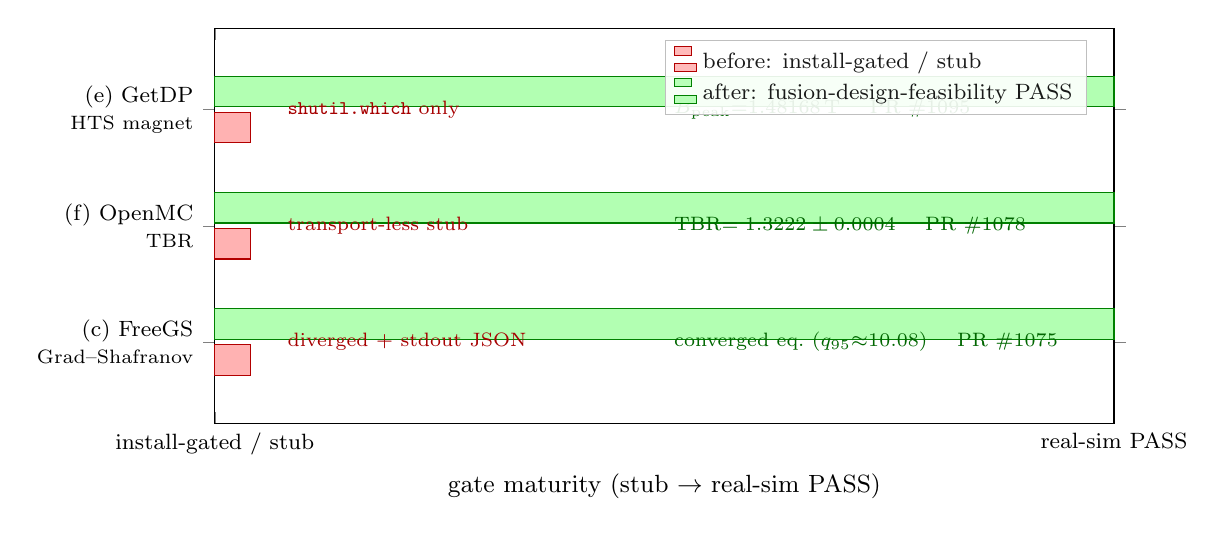
\begin{tikzpicture}
\begin{axis}[
  width=13cm, height=6.6cm,
  xbar,
  bar width=11pt,
  xmin=0, xmax=1.0,
  xtick={0,1}, xticklabels={install-gated / stub, real-sim PASS},
  x tick label style={font=\footnotesize},
  ytick={1,2,3},
  yticklabels={%
    \shortstack[r]{(c) FreeGS\\\scriptsize Grad--Shafranov},
    \shortstack[r]{(f) OpenMC\\\scriptsize TBR},
    \shortstack[r]{(e) GetDP\\\scriptsize HTS magnet}},
  y tick label style={font=\footnotesize,align=right},
  ymin=0.3, ymax=3.7,
  xlabel={gate maturity (stub $\to$ real-sim PASS)},
  label style={font=\small},
  xmajorgrids,
  grid style={gray!25},
  enlarge y limits=0.0,
  clip=false,
  legend pos=north east,
  legend cell align=left,
  legend style={font=\footnotesize,fill=white,fill opacity=0.9,draw=gray!50},
]
% before: install-gated stub state (x=0, drawn as a tiny stub marker bar)
\addplot[draw=red!70!black,fill=red!30] coordinates {
  (0.04,1) (0.04,2) (0.04,3)
};
\addlegendentry{before: install-gated / stub}
% after: real-sim PASS (x=1)
\addplot[draw=green!50!black,fill=green!30] coordinates {
  (1,1) (1,2) (1,3)
};
\addlegendentry{after: fusion-design-feasibility PASS}
% per-gate after-state result + PR label
\node[font=\scriptsize,text=green!40!black,anchor=west] at (axis cs:0.50,3)
  {$B_{\mathrm{peak}}{=}1.48168$\,T \quad PR \#1095};
\node[font=\scriptsize,text=green!40!black,anchor=west] at (axis cs:0.50,2)
  {TBR$=1.3222\pm0.0004$ \quad PR \#1078};
\node[font=\scriptsize,text=green!40!black,anchor=west] at (axis cs:0.50,1)
  {converged eq.\ ($q_{95}{\approx}10.08$) \quad PR \#1075};
% before-state defect label
\node[font=\scriptsize,text=red!65!black,anchor=west] at (axis cs:0.07,3)
  {\texttt{shutil.which} only};
\node[font=\scriptsize,text=red!65!black,anchor=west] at (axis cs:0.07,2)
  {transport-less stub};
\node[font=\scriptsize,text=red!65!black,anchor=west] at (axis cs:0.07,1)
  {diverged + stdout JSON};
\end{axis}
\end{tikzpicture}
\end{document}
